\documentclass[../../main.tex]{subfiles}

\begin{document}

En este apéndice se describe todo el proceso de instalación de la aplicación bajo cualquier ordenador y sistema operativo. \\
Antes de entrar en los detalles es necesario remarcar, que se precisa de un ordenador con unas características con una configuración mínima que se detallan a continuación para que se pueda ejecutar la aplicación sin problemas:
\begin{enumerate}
\item Procesador: Intel Core i5 o AMD Ryzen 5
\item Memoria RAM: 8 GB
\item Disco SSD
\end{enumerate}

El siguiente paso es descargar el código fuente del repositorio ubicado en \Gls{github}, abrimos la página del  \href{https://github.com/beaudryjp/sna_fcaR}{repositorio} y aparecerá una pantalla similar a la siguiente:

\begin{figure}[h]
\centering
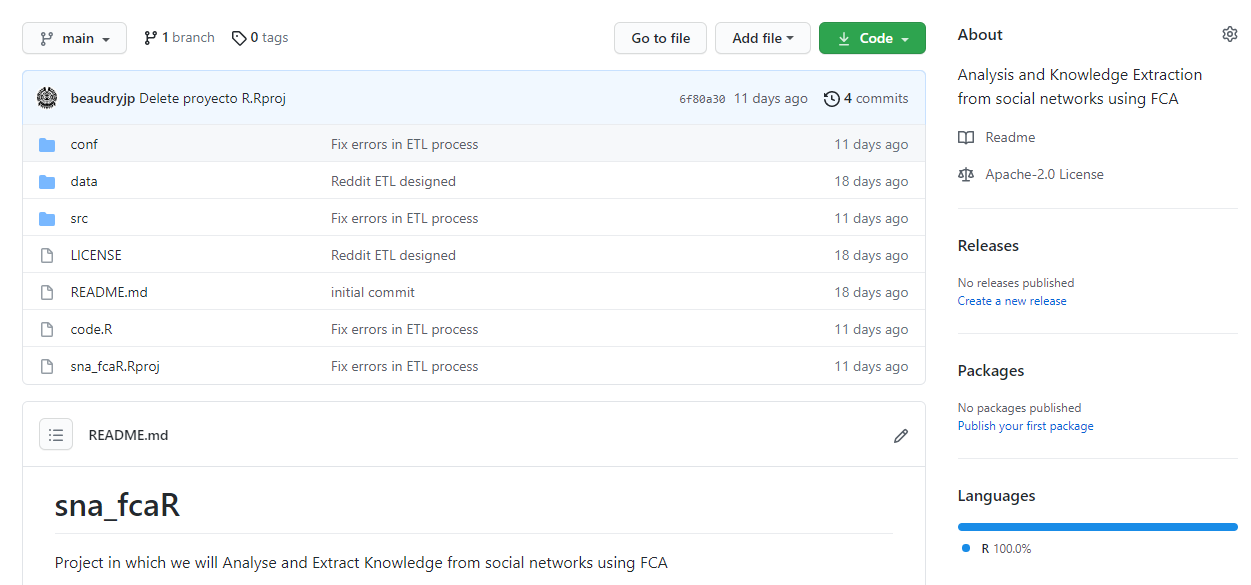
\includegraphics[width=\textwidth]{images/apendices/github1.png}
\caption{Repositorio del código fuente de la aplicación}
\end{figure}

En dicha pantalla hay que pulsar sobre el botón \textit{CODE} y posteriormente \textit{Download ZIP}, esto descargará un fichero comprimido con todo el código fuente del proyecto el cual puede ser abierto por las aplicaciones nativas de descompresión de ficheros de cualquier sistema operativo. \\


Para el siguiente paso es necesario disponer de un servidor de base de datos ya existente o instalar uno nuevo, para este presente trabajo se utiliza la herramienta \Gls{docker}\cite{doc10}, el cual gestionará dos contenedores, una maquina virtual con el servidor de base de datos \gls{mariadb}\cite{doc11} y una maquina virtual con el gestor de base de datos \gls{phpmyadmin}\cite{doc12} ya preconfigurada.\\

\textit{NOTA: } Si la instalación se hace bajo el sistema operativo Windows, es necesario disponer de la versión 10 del mismo y tener instalado el Subsistema de Linux para Windows.
En el siguiente \href{https://docs.microsoft.com/en-us/windows/wsl/install-win10}{enlace} viene detallado los pasos a seguir para la instalación de dicho subsistema.\\

Se recomienda instalar \Gls{docker} con las opciones que aparecen por defecto, una vez instalado la aplicación Docker, es necesario abrir una ventana de terminal (En Linux/MacOS: Terminal, En Windows: \gls{powershell}) y ejecutar los siguientes comandos en el siguiente orden:

\begin{itemize}
\item Para el contenedor \gls{mariadb} con los  parámetros:
\begin{itemize}
\item[$\ast$] \textit{-p}: El puerto interno y externo en el que corre el servicio \gls{mariadb}.
\item[$\ast$]\textit{-name}: El nombre del contenedor.
\item[$\ast$] \textit{-e}: Establecemos como variable de entorno la contraseña del usuario \textbf{root}, remarcar que es recomendable cambiar la contraseña a una más segura si se pone la aplicación en producción.
\item[$\ast$] \textit{-d}: Indicar que el contenedor funcione en segundo plano.
\end{itemize}
\end{itemize}
\begin{lstlisting}
docker run -p 3306:3306  --name mariadb -e MYSQL_ROOT_PASSWORD=root123 -d mariadb/server
\end{lstlisting}

\vskip 0.2in

\begin{itemize}
\item Para el contenedor \gls{phpmyadmin} con los parámetros:
\begin{itemize}
\item[$\ast$] \textit{-p}: El puerto interno y externo en el que corre el servicio \gls{phpmyadmin}.
\item[$\ast$]\textit{-name}: El nombre del contenedor.
\item[$\ast$] \textit{--link}: Enlazamiento de este contenedor con el contenedor del servidor de base de datos \gls{mariadb}.
\item[$\ast$] \textit{-d}: Indicar que el contenedor funcione en segundo plano.
\end{itemize}
\end{itemize}
\begin{lstlisting}
docker run --name my-own-phpmyadmin -d --link mariadb:db -p 8081:80 phpmyadmin/phpmyadmin
\end{lstlisting}

\vskip 0.2in

Una vez ejecutados estos dos comandos, tendremos dos contenedores con dos servicios diferentes en funcionamiento y en segundo plano. Para acceder al gestor de base datos hay que abrir un navegador y acceder a la siguiente dirección \href{127.0.0.1:8081}{127.0.0.1:8081}, pinchar en la pestaña \textit{\gls{sql}} y pegar el contenido copiado anteriormente. \\

En este momento es necesario crear la base de datos en la cual se alojará los datos relativos a la aplicación, este proceso se puede realizar mediante el gestor de base de datos \textit{\gls{phpmyadmin}} en la pestaña \textit{Databases}.

\begin{figure}[H]
\centering
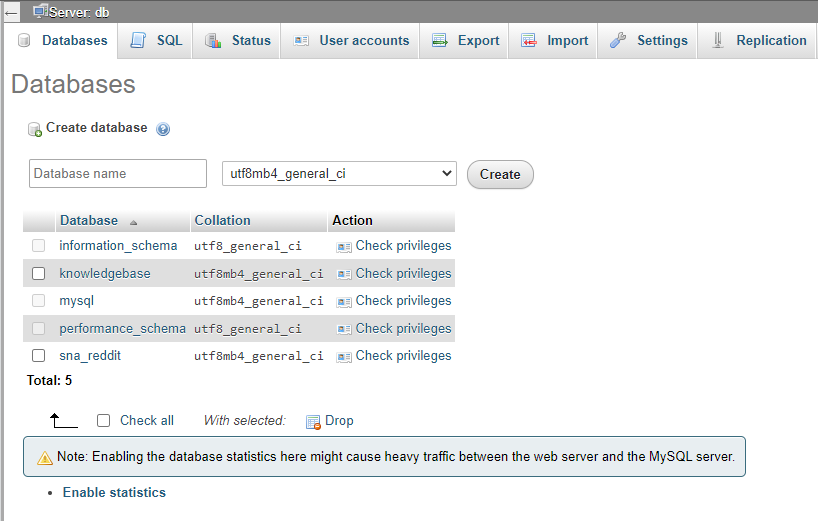
\includegraphics[width=\textwidth]{images/apendices/phpmyadmin-1.png}
\caption{Gestor de Base de datos - Creación nueva base de datos}
\end{figure}

No obstante también es posible realizarlo mediante un comando, el cual se especifica a continuación:

\begin{lstlisting}
docker exec -it mariadb mysql -uroot -proot123 -e "create database sna_reddit"
\end{lstlisting}

\vskip 0.2in

Para este presente proyecto se ha creado un usuario para el servidor de base de datos llamado \textit{david}, tal como se ha realizado en el punto anterior también es posible realizarlo por el gestor de base de datos \textit{phpMyAdmin} en la pestaña \textit{Privileges}. 

\begin{figure}[H]
\centering
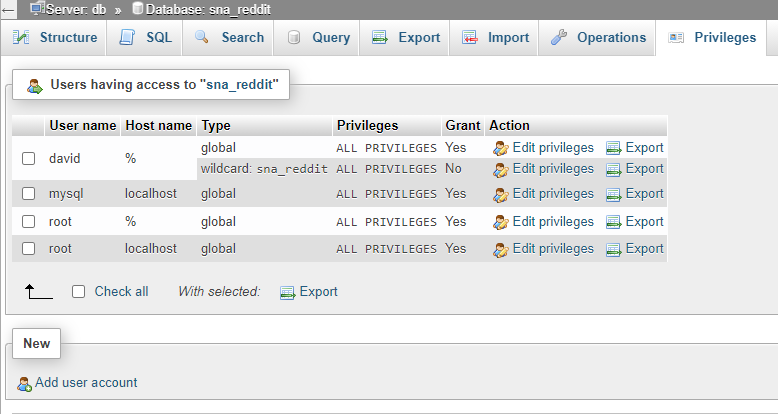
\includegraphics[width=\textwidth]{images/apendices/phpmyadmin-2.png}
\caption{Gestor de Base de datos - Creación nuevo usuario}
\end{figure}

Igualmente es posible realizarlo mediante un comando para la consola, el cual se especifica a continuación:

\begin{lstlisting}
docker exec -it mariadb mysql -uroot -proot123 -e "CREATE USER 'david'@'%' IDENTIFIED BY 'p1YFHaVBpDmmurLU';"

docker exec -it mariadb mysql -uroot -proot123 -e "GRANT ALL PRIVILEGES on sna_reddit.* TO 'david'@'%' IDENTIFIED BY 'p1YFHaVBpDmmurLU'; FLUSH PRIVILEGES;"
\end{lstlisting}

\vskip 0.2in

Para importar la copia de seguridad de la base de datos en el servidor es recomendable realizarlo mediante línea de comandos debido al gran tamaño que tiene el fichero, no obstante esta operación se puede realizar mediante la aplicación web \textit{\gls{phpmyadmin}}. Para realizarlo mediante la consola es necesario abrir una y ejecutar el siguiente comando:

\begin{lstlisting}
docker exec -i mariadb mysql -uroot -proot123 sna_reddit < "sna_reddit.sql"
\end{lstlisting}

Por último, comentar que es posible encadenar la ejecución de todos estos comandos en uno solo para una mayor facilidad en la mantenimiento y administración de este servidor de base de datos:

\begin{lstlisting}
docker run -p 3306:3306 --network r-db --name mariadb -e MYSQL_ROOT_PASSWORD=root123 -d mariadb/server && sleep 5 && \
  docker exec -it mariadb mysql -uroot -proot123 -e "create database sna_reddit" && sleep 5 && \
  docker exec -it mariadb mysql -uroot -proot123 -e "CREATE USER 'david'@'%' IDENTIFIED BY 'p1YFHaVBpDmmurLU'; " && sleep 5 &&
  docker exec -it mariadb mysql -uroot -proot123 -e "GRANT ALL PRIVILEGES on sna_reddit.* TO 'david'@'%' IDENTIFIED BY 'p1YFHaVBpDmmurLU'; FLUSH PRIVILEGES;" && sleep 5 && \
  docker exec -i mariadb mysql -uroot -proot123 sna_reddit < "sna_reddit.sql" && sleep 5 && \
  docker run --name mariadb-phpmyadmin --network r-db -d --link mariadb:db -p 8081:80 phpmyadmin/phpmyadmin
\end{lstlisting}

\vskip 0.2in

Donde hay que especificar la contraseña root correcta en todas las operaciones que se realizan por la consola referente al servidor de base de datos. \\

Ahora creamos una imagen modificada de la aplicación web \Gls{shiny} que incluye los paquetes necesarios para que la aplicación funcione, esta configuración viene definido en el fichero \textit{\Gls{dockerfile}} que se encuentra ubicado en la carpeta data.

Debemos crear una nueva carpeta en la cual tenemos la siguiente estructura:
\begin{itemize}
\item app/ (carpeta dónde estará ubicada el código fuente de la aplicación)
\item \Gls{dockerfile} (fichero con la configuración \Gls{docker})
\end{itemize}

Una vez se tiene esta estructura es necesario abrir una consola y ejecutar el siguiente comando:
\begin{lstlisting}
docker build --tag custom-shiny .
\end{lstlisting}

\vskip 0.2in

Al finalizar la ejecución de este comando aparecerá si se ha ejecutado de forma correcta o no, en caso de que no ha habido problemas procedemos a lanzar el siguiente comando para crear un contendedor basado en esta nueva imagen creada:
\begin{lstlisting}
docker run -d --name rshiny -p 3838:3838 custom-shiny 
\end{lstlisting}

\vskip 0.2in

Con esto ya es posible acceder a la aplicación \Gls{shiny} mediante un navegador web mediante el enlace \href{127.0.0.1:3838}{127.0.0.1:3838}. \\

Con respecto al funcionamiento de los contenedores, es posible visualizar si están funcionando de forma correcta con el siguiente comando:

\begin{lstlisting}
docker ps -a
\end{lstlisting}

\vskip 0.2in

Para ver el consumo actual de cada contenedor, es necesario ejecutar el siguiente comando:

\begin{lstlisting}
docker stats
\end{lstlisting}

\end{document}